\documentclass[a4paper,11pt]{article}
\usepackage[utf8]{inputenc}
\usepackage[margin=2.5cm]{geometry}
\usepackage{graphicx}
\usepackage{float}
\usepackage{listings}
\usepackage{xcolor}
\usepackage{longtable}
\usepackage{array}
\usepackage{hyperref}
\usepackage{amssymb}
\usepackage{amsmath}
\graphicspath{{doc/}{./}}

% Definisi Warna
\definecolor{codegreen}{rgb}{0,0.6,0}
\definecolor{codegray}{rgb}{0.5,0.5,0.5}
\definecolor{codepurple}{rgb}{0.58,0,0.82}
\definecolor{backcolour}{rgb}{0.95,0.95,0.92}

% Definisi Style Listing
\lstdefinestyle{mystyle}{
    backgroundcolor=\color{backcolour},
    commentstyle=\color{codegreen},
    keywordstyle=\color{blue}\bfseries,
    numberstyle=\tiny\color{codegray},
    stringstyle=\color{codepurple},
    basicstyle=\ttfamily\footnotesize,
    breakatwhitespace=false,
    breaklines=true,
    captionpos=b,
    keepspaces=true,
    numbers=left,
    numbersep=5pt,
    showspaces=false,
    showstringspaces=false,
    showtabs=false,
    tabsize=2
}

\lstset{style=mystyle}

\lstdefinelanguage{Pseudocode}{
    keywords={FUNCTION, ALGORITMA, KAMUS, LOKAL, IF, THEN, ELSE, RETURN, FOR, TO, DO, WHILE, TYPE, LIST, of, AND, OR, NOT, input, output, true, false, null, push, pop},
    sensitive=true,
    morecomment=[s]{\{}{\}},
    morestring=[b]",
}

\begin{document}

% ===== HALAMAN JUDUL (COVER) =====
\begin{titlepage}
\centering
\vspace*{1cm}

% ===== Header =====
{\fontsize{14pt}{16pt}\selectfont\textbf{IF2211 - K01}}\\[1cm]

{\fontsize{16pt}{18pt}\selectfont\textbf{TUGAS KECIL 3 STRATEGI ALGORITMA}}\\[0.5cm]

{\fontsize{12pt}{14pt}\selectfont
Penyelesaian Permainan Ice Sliding Puzzle dengan Menggunakan Algoritma Pathfinding
}\\[2cm]

% ===== Logo =====
\IfFileExists{cover.png}{
    
\includegraphics[width=0.5\textwidth]{cover.png}\\[2cm]
}{
    \vspace{3cm}
}

% ===== Penyusun =====
{\fontsize{12pt}{14pt}\selectfont Disusun oleh:}\\[0.5cm]

{\fontsize{12pt}{14pt}\selectfont
\begin{tabular}{c c}
Raymond Jonathan Dwi Putra Julianto & 13524059
\end{tabular}
}

\vfill

% ===== Footer =====
{\fontsize{14pt}{16pt}\selectfont\textbf{SEKOLAH TEKNIK ELEKTRO DAN INFORMATIKA}}\\[0.5cm]
{\fontsize{14pt}{16pt}\selectfont\textbf{INSTITUT TEKNOLOGI BANDUNG}}\\[0.5cm]

{\fontsize{14pt}{16pt}\selectfont 2026}

\vspace*{1cm}
\end{titlepage}

\setcounter{page}{1}
\tableofcontents
\newpage

\section{Permasalahan}
Ice Sliding Puzzle adalah permainan pencarian jalur pada papan dua dimensi. Pemain atau aktor berada pada satu titik awal dan harus mencapai titik tujuan. Berbeda dengan pergerakan biasa, aktor tidak bergerak satu petak lalu berhenti. Ketika aktor memilih arah atas, kanan, bawah, atau kiri, aktor akan terus meluncur pada arah tersebut sampai berhenti tepat sebelum rintangan.

Pada papan permainan terdapat beberapa jenis tile. Tile \texttt{Z} menyatakan posisi awal aktor, tile \texttt{O} menyatakan posisi tujuan, tile \texttt{X} menyatakan rintangan, tile \texttt{L} menyatakan lava, tile \texttt{*} menyatakan jalan biasa, dan tile angka \texttt{0} sampai \texttt{9} menyatakan tile penting. Tile angka harus dilewati sesuai urutan dari angka terkecil. Apabila aktor melewati angka yang lebih besar sebelum waktunya, jalur tersebut dianggap tidak valid. Apabila aktor melewati lava atau bergerak keluar papan tanpa dapat berhenti, jalur tersebut juga dianggap tidak valid.

\section{Pendekatan Solusi}
Permasalahan ini diselesaikan dengan pendekatan \textit{graph search}. Papan permainan terlebih dahulu dibaca sebagai objek \texttt{Board}. Setelah itu, program membentuk graph sederhana. Node pada graph bukan semua tile di papan, melainkan hanya posisi yang dapat menjadi tempat aktor berhenti setelah melakukan sliding. Dengan demikian, satu edge pada graph mewakili satu gerakan sliding lengkap dari satu posisi berhenti ke posisi berhenti lain.

Setiap edge menyimpan arah gerak, node tujuan, cost total tile yang dilalui, dan daftar tile penting yang dilewati selama sliding. Pendekatan ini penting karena tile angka atau finish dapat berada di tengah lintasan sliding. Apabila tile penting berada di tengah lintasan tetapi aktor tidak berhenti di sana, tile tersebut tidak menjadi node tujuan, tetapi tetap dicatat sebagai tile yang dilewati pada edge. Informasi ini kemudian digunakan saat pathfinding untuk memvalidasi urutan angka.

Sebagai contoh, misalkan terdapat potongan papan sebagai berikut. Simbol \texttt{Z} adalah posisi awal, \texttt{O} adalah finish, \texttt{0} adalah tile penting, dan \texttt{X} adalah rintangan.

\begin{lstlisting}[caption=Contoh Board Sederhana]
XXXXXXX
X0***OX
X**X**X
X****XX
XZ***XX
XXXXXXX
\end{lstlisting}

Pada representasi board biasa, setiap karakter pada matriks adalah tile. Namun pada graph sederhana, tidak semua tile menjadi node. Pembuatran Node hanya dibuat pada posisi yang dapat menjadi tempat aktor berhenti. Dari posisi awal \texttt{Z}, aktor dapat melakukan sliding ke atas sampai berhenti tepat sebelum rintangan atau melakukan sliding ke kanan sampai berhenti sebelum rintangan. Tile yang hanya dilewati di tengah lintasan tidak otomatis menjadi node.

Sebagai ilustrasi, beberapa node yang terbentuk dapat direpresentasikan seperti berikut.

\begin{longtable}{|c|c|c|p{6cm}|}
    \hline
    \textbf{Node} & \textbf{Posisi} & \textbf{Tile} & \textbf{Alasan Menjadi Node} \\
    \hline
    \endhead
    N0 & Baris 4, Kolom 1 & \texttt{Z} & Posisi awal aktor. \\
    \hline
    N1 & Baris 1, Kolom 1 & \texttt{0} & Hasil slide ke atas dari \texttt{Z} dan berhenti sebelum dinding atas. \\
    \hline
    N2 & Baris 4, Kolom 4 & \texttt{*} & Hasil slide ke kanan dari \texttt{Z} dan berhenti sebelum rintangan. \\
    \hline
    N3 & Baris 1, Kolom 5 & \texttt{O} & Posisi finish yang dapat menjadi posisi berhenti. \\
    \hline
\end{longtable}

Dari node-node tersebut, edge menyimpan satu gerakan sliding penuh. Contohnya, apabila dari \texttt{Z} aktor bergerak ke atas, maka edge yang terbentuk adalah \texttt{N0 -> N1} dengan arah \texttt{U}. Apabila dari \texttt{N1} aktor bergerak ke kanan dan melewati beberapa tile kosong sampai berhenti di \texttt{O}, maka edge yang terbentuk adalah \texttt{N1 -> N3} dengan arah \texttt{R}. Jika di tengah edge terdapat angka yang dilewati, angka tersebut disimpan pada \texttt{passedImportant}, bukan dipaksa menjadi node baru kecuali aktor memang berhenti tepat di tile tersebut.

\subsection{Konsep Algoritma}
Secara umum, proses pencarian solusi dibagi menjadi tiga tahap utama. Tahap pertama adalah membaca dan memvalidasi input. Tahap kedua adalah membangun graph sederhana dari papan. Tahap ketiga adalah menjalankan algoritma pencarian pada graph tersebut.

\subsubsection{Tahap 1: Pembacaan Board}
Tahap pertama dilakukan oleh fungsi \texttt{readBoardFromFile}. Fungsi ini menerima sebuah path file teks dan mengembalikan objek \texttt{Board} yang sudah berisi data tile beserta cost. Pembacaan dilakukan dalam urutan sebagai berikut.

\begin{enumerate}
    \item Membaca dua bilangan bulat pertama yang menyatakan jumlah baris ($R$) dan jumlah kolom ($C$) papan. Apabila salah satu nilai tidak valid atau bukan bilangan positif, program melempar error.
    \item Membaca $R$ baris berikutnya sebagai matriks tile. Setiap baris harus memiliki panjang tepat $C$ karakter. Setiap karakter harus berasal dari himpunan tile yang valid, yaitu \texttt{*}, \texttt{X}, \texttt{L}, \texttt{Z}, \texttt{O}, atau angka \texttt{0}--\texttt{9}.
    \item Selama pembacaan tile, program menghitung jumlah \texttt{Z} dan \texttt{O} serta menyimpan angka tile penting yang muncul. Posisi \texttt{Z} disimpan sebagai start dan posisi \texttt{O} disimpan sebagai goal.
    \item Setelah seluruh tile dibaca, program membaca matriks cost berukuran $R \times C$. Setiap nilai cost wajib berupa bilangan bulat tidak negatif.
    \item Setelah seluruh data dibaca, program melakukan validasi akhir. Jumlah \texttt{Z} harus tepat satu, jumlah \texttt{O} harus tepat satu, dan angka tile penting harus berurutan mulai dari \texttt{0} hingga maksimum yang ditemukan tanpa ada yang loncat. Jumlah angka penting kemudian disimpan sebagai \texttt{importantCount}.
\end{enumerate}

Pembacaan dilakukan secara linier sehingga kompleksitasnya adalah $O(R \times C)$, sama dengan ukuran input. Karena validasi dilakukan saat baris dan cost diparse, kesalahan format dapat dideteksi sedini mungkin.

\begin{lstlisting}[language=Pseudocode, caption=Pseudocode Pembacaan dan Validasi Board, label={lst:readboard}]
FUNCTION ReadBoardFromFile(filePath) -> board
ALGORITMA
    input <- buka file pada filePath
    IF input gagal dibuka THEN
        throw error "file tidak dapat dibuka"

    baca rowCount, colCount dari input
    IF rowCount <= 0 OR colCount <= 0 THEN
        throw error "ukuran peta tidak valid"

    board <- Board(rowCount, colCount)
    startCount <- 0
    goalCount <- 0
    foundNumbers <- array boolean berukuran 10, semuanya false
    maxNumber <- -1

    FOR row dari 0 TO rowCount - 1 DO
        baca line dari input
        IF panjang(line) != colCount THEN
            throw error "panjang baris tidak sesuai"

        FOR col dari 0 TO colCount - 1 DO
            type <- line[col]
            IF type bukan tile yang valid THEN
                throw error "karakter peta tidak valid"

            IF type == 'Z' THEN
                startCount <- startCount + 1
            ELSE IF type == 'O' THEN
                goalCount <- goalCount + 1
            ELSE IF type adalah angka THEN
                foundNumbers[type - '0'] <- true
                maxNumber <- max(maxNumber, type - '0')

            board.setType(row, col, type)

    FOR row dari 0 TO rowCount - 1 DO
        FOR col dari 0 TO colCount - 1 DO
            baca cost dari input
            IF cost < 0 THEN
                throw error "cost peta tidak valid"
            board.setCost(row, col, cost)

    IF startCount != 1 THEN
        throw error "harus tepat satu Z"
    IF goalCount != 1 THEN
        throw error "harus tepat satu O"

    FOR number dari 0 TO maxNumber DO
        IF foundNumbers[number] == false THEN
            throw error "angka harus berurutan mulai dari 0"

    board.importantCount <- maxNumber + 1
    RETURN board
\end{lstlisting}

\subsubsection{Tahap 2: Pembentukan Graph}
Setelah \texttt{Board} terbentuk, tahap kedua adalah membangun graph sederhana. Pada graph ini, node hanya dibuat untuk posisi yang dapat menjadi tempat aktor berhenti, sedangkan edge menyatakan satu gerakan sliding lengkap. Pembentukan dilakukan dengan BFS bermula dari posisi \texttt{Z}. Untuk setiap node, fungsi \texttt{slide} dipanggil dengan empat arah gerak. Hasil sliding yang valid menghasilkan node tujuan baru (atau menggunakan node yang sudah ada apabila posisinya sama) beserta edge baru yang menyimpan arah, cost total, dan daftar tile penting yang dilewati. Setelah seluruh node selesai dieksplorasi, fungsi \texttt{setPredictionCosts} dipanggil untuk menghitung nilai jarak Manhattan dari setiap node menuju goal dan menuju setiap angka penting. Nilai-nilai ini akan dipakai sebagai heuristic pada GBFS dan A*.

\begin{lstlisting}[language=Pseudocode, caption=Pseudocode Pembentukan Graph Sederhana, label={lst:buildgraph}]
FUNCTION BuildGraph(board) -> graph
ALGORITMA
    root <- node pada posisi start Z
    frontier.push(root)
    processed <- empty set

    WHILE frontier tidak kosong DO
        current <- frontier.pop()
        IF current sudah ada di processed THEN
            continue
        processed.insert(current)

        FOR setiap arah gerak DO
            slideResult <- Slide(board, current, arah)
            IF slideResult tidak valid THEN
                continue

            nextNode <- node pada posisi berhenti slideResult
            IF nextNode belum ada THEN
                tambahkan nextNode ke graph
                frontier.push(nextNode)

            tambahkan edge current -> nextNode
            simpan arah, cost, dan passedImportant pada edge

    hitung nilai heuristic setiap node
    RETURN graph
\end{lstlisting}

\subsubsection{Tahap 3: Pencarian Solusi}
Setelah graph terbentuk, pencarian dilakukan dengan state yang tidak hanya menyimpan posisi node, tetapi juga angka berikutnya yang harus dilewati. Hal ini dibutuhkan karena dua jalur dapat berhenti pada node yang sama tetapi memiliki progres angka yang berbeda.

State pencarian didefinisikan sebagai pasangan $(nodeId, nextNumber)$. Variabel $nodeId$ menyatakan posisi berhenti aktor pada graph, sedangkan $nextNumber$ menyatakan indeks angka penting berikutnya yang masih harus dilewati. Dengan struktur ini, dua kunjungan terhadap node yang sama dengan progres angka yang berbeda diperlakukan sebagai dua state yang berbeda. Tabel \texttt{bestCost[(nodeId, nextNumber)]} digunakan untuk mencatat cost terbaik yang pernah ditemukan pada setiap state, sehingga state dengan cost lebih buruk tidak ikut diperluas. Ekspansi suatu state dilakukan dengan menelusuri seluruh edge yang keluar dari $nodeId$. Untuk setiap edge, daftar \texttt{passedImportant} dievaluasi secara berurutan. Bila edge melewati angka yang lebih besar dari $nextNumber$, edge tersebut dianggap tidak valid karena melanggar urutan. Bila edge melewati angka yang sama atau lebih kecil, $nextNumber$ diperbarui sehingga state berikutnya menyimpan progres yang sudah diperhitungkan. Disini, iterasi pada program direpresentasikan sebagai melakukannya satu kali sliding atau berpindahnya node yang ada sebanyak satu kali.

\begin{lstlisting}[language=Pseudocode, caption=Pseudocode Pathfinding, label={lst:pathfinding}]
FUNCTION Search(graph, algorithm, heuristicMode) -> solution
ALGORITMA
    rootState <- (rootNode, nextNumber = 0, g = 0)
    frontier.push(rootState)
    bestCost[rootNode, 0] <- 0

    WHILE frontier tidak kosong DO
        current <- frontier.pop dengan prioritas terbaik

        IF current berada di O AND semua angka selesai THEN
            RETURN path dari start ke current

        FOR setiap edge dari current.node DO
            nextNumber <- current.nextNumber
            valid <- ApplyPassedImportant(edge.passedImportant, nextNumber)
            IF NOT valid THEN
                continue

            newCost <- current.g + edge.cost
            IF newCost lebih baik dari bestCost[edge.to, nextNumber] THEN
                hitung priority sesuai UCS, GBFS, atau A*
                frontier.push(state baru)

    RETURN tidak ada solusi
\end{lstlisting}

Pada implementasi ini, ketiga algoritma tidak ditulis sebagai tiga fungsi yang terpisah. Ketiganya berjalan pada satu fungsi internal \texttt{search} dengan struktur kerja yang sama: state $(nodeId, nextNumber)$, tabel \texttt{bestCost} untuk pruning, satu \texttt{priority\_queue} dengan field \texttt{priority}, pengecekan goal saat pop, validasi urutan angka pada setiap edge, serta rekonstruksi path melalui rantai \texttt{HistoryRecord}. Yang membedakan UCS, GBFS, dan A* hanya cara mengisi field \texttt{priority} dan apakah $h(n)$ perlu dihitung. Pemilihan rumus \texttt{priority} ditangani oleh sebuah lambda \texttt{priorityFor(gCost, heuristicCost)} yang mengembalikan nilai berbeda sesuai parameter \texttt{algorithm}. Berikut penjelasan langsung bagaimana setiap algoritma bekerja di dalam fungsi yang sama.

Pada UCS, parameter \texttt{algorithm} bernilai \texttt{Algorithm::UCS} sehingga \texttt{priorityFor} mengembalikan \texttt{gCost} saja. Fungsi \texttt{search} juga sengaja melewati pemanggilan \texttt{getHeuristicCost} dan langsung mengisi \texttt{heuristicCost = 0} karena heuristic tidak diperlukan. Akibatnya, state diambil dari priority queue selalu dalam urutan menaik berdasarkan cost aktual dari \texttt{Z}.

Pada GBFS, parameter \texttt{algorithm} bernilai \texttt{Algorithm::GBFS} sehingga \texttt{priorityFor} mengembalikan \texttt{heuristicCost} saja. Nilai \texttt{heuristicCost} diisi oleh \texttt{Graph::getHeuristicCost(node, nextNumber, mode)} sesuai mode H1, H2, atau H3 yang dipilih pengguna. Karena \texttt{gCost} tidak ikut diperhitungkan, GBFS akan mengambil state yang terlihat paling dekat dengan target dari priority queue, walaupun cost untuk sampai ke state tersebut sudah besar. Hal ini membuat GBFS sering kali cepat menemukan solusi pertama, namun solusi tersebut belum tentu memiliki cost terkecil karena ekspansi tidak mempertimbangkan jarak yang sudah ditempuh.

Pada A*, parameter \texttt{algorithm} bernilai \texttt{Algorithm::AStar} sehingga \texttt{priorityFor} mengembalikan \texttt{gCost + heuristicCost}, yaitu $f(n) = g(n) + h(n)$. Sama seperti GBFS, nilai \texttt{heuristicCost} diisi melalui \texttt{Graph::getHeuristicCost} sesuai mode H1, H2, atau H3.

Rekonstruksi path dilakukan setelah goal ditemukan dengan menelusuri rantai \texttt{HistoryRecord} dari state goal ke state awal secara mundur, kemudian dibalik agar menghasilkan urutan langkah dari awal ke akhir.

\subsection{Heuristic}
\label{subsec:heuristic}
Untuk GBFS dan A*, program menyediakan tiga mode heuristic. Ketiga mode bekerja pada level node graph, bukan pada tile mentah, dan seluruhnya menggunakan jarak Manhattan sebagai dasar perhitungan. Dengan node $n$ berada di posisi $(r_n, c_n)$, jarak Manhattan ke target di posisi $(r_t, c_t)$ didefinisikan sebagai
\[
d(n, t) = |r_n - r_t| + |c_n - c_t|.
\]

\textbf{H1 FinishOnly.} Heuristic H1 hanya melihat jarak Manhattan dari node saat ini menuju tile finish \texttt{O}. Secara matematis, $h_1(n) = d(n, O)$. Heuristic ini paling sederhana dan tidak peduli pada angka penting yang belum dilewati. Karena hanya memperhatikan finish, H1 berperilaku baik pada peta tanpa angka penting atau pada saat seluruh angka sudah dilewati. Pada peta dengan banyak angka, H1 dapat menyesatkan karena pencarian akan terdorong ke arah finish meskipun aktor masih harus berputar mengambil angka. Pada implementasi, nilai $h_1$ sudah dihitung saat pembentukan graph dan disimpan sebagai \texttt{finishPredictionCost} pada setiap node.

\textbf{H2 ImportantSequence.} Heuristic H2 mengarahkan pencarian ke angka berikutnya yang harus dilewati. Diberikan state $(node, nextNumber)$ dengan jumlah angka penting $K$, heuristic dihitung sebagai
\[
h_2(n) =
\begin{cases}
d(n, T_{nextNumber}) & \text{jika } nextNumber < K, \\
d(n, O) & \text{jika } nextNumber = K,
\end{cases}
\]
dengan $T_i$ adalah posisi angka penting $i$. Selama angka belum habis, H2 fokus mempersempit jarak ke angka berikutnya, sehingga lebih informatif daripada H1 di tahap awal pencarian. Setelah seluruh angka dilewati, H2 otomatis berperilaku seperti H1, yaitu menarik aktor ke finish. Karena hanya menjumlah satu jarak Manhattan, H2 cenderung menjadi nilai estimasi yang relatif kecil, sehingga lebih aman terhadap pelanggaran admissibility dibanding H3.

\textbf{H3 OrderedSequence.} Heuristic H3 mencoba memperkirakan total perjalanan yang masih tersisa dengan menjumlahkan jarak Manhattan ke seluruh target yang belum dilewati secara berurutan, lalu ke finish. Diberikan state $(node, nextNumber)$ dengan posisi $T_{nextNumber}, T_{nextNumber+1}, \dots, T_{K-1}, O$ sebagai rangkaian target yang masih harus dilewati, heuristic dihitung sebagai
\[
h_3(n) = d(n, T_{nextNumber}) + \sum_{i = nextNumber}^{K-2} d(T_i, T_{i+1}) + d(T_{K-1}, O).
\]
Apabila seluruh angka sudah selesai, $h_3$ langsung sama dengan $d(n, O)$. H3 paling informatif karena memperhitungkan beban perjalanan dari posisi sekarang ke seluruh target dan kemudian ke finish. Pengaruhnya jelas terlihat pada GBFS, di mana H3 sering memilih jalur yang mempertimbangkan urutan angka dengan lebih baik dibanding H1 atau H2. Namun, karena nilai estimasi H3 dapat menjadi cukup besar, H3 lebih rentan kehilangan sifat admissibility, sehingga A* dengan H3 tidak selalu menjamin solusi optimal walaupun pada banyak peta tetap mendekati optimal.

\section{Analisis Algoritma}
\subsection{Definisi State, \texorpdfstring{$g(n)$}{g(n)}, dan \texorpdfstring{$f(n)$}{f(n)}}
\label{subsec:state-def}

Ruang state pada Ice Sliding Puzzle tidak cukup hanya direpresentasikan sebagai posisi aktor. Karena ada aturan urutan tile penting yang harus dipatuhi, dua situasi berbeda dapat terjadi pada posisi papan yang sama: satu sudah mengambil checkpoint tertentu dan satu lagi belum. Kedua situasi ini harus diperlakukan berbeda oleh algoritma karena transisi yang diperbolehkan pun berbeda.

Oleh karena itu, state pencarian didefinisikan sebagai pasangan:
\[
s = (nodeId,\; nextNumber),
\]
dengan $nodeId$ menyatakan indeks node pada graph sederhana (posisi berhenti aktor) dan $nextNumber$ menyatakan indeks angka penting berikutnya yang wajib dilewati ($0 \leq nextNumber \leq K$ dengan $K$ adalah total tile angka pada peta). State awal adalah $(root,\; 0)$ dan state goal adalah semua state $(n,\; K)$ di mana $n$ adalah node bertipe \texttt{O}.

Nilai $g(n)$ didefinisikan sebagai total cost aktual dari state awal menuju state $n$, yaitu jumlah cost seluruh tile yang dilalui pada setiap gerakan sliding sepanjang jalur. Karena satu edge mewakili satu sliding penuh yang dapat melewati banyak tile, cost sebuah edge dihitung sebagai akumulasi cost seluruh tile yang dilintasi, bukan hanya tile tujuan. Secara rekursif:
\[
g(n') = g(n) + c(n, n'),
\]
dengan $c(n, n')$ adalah cost edge dari $n$ ke $n'$. Oleh karena itu, $g(n) \geq 0$ selalu terpenuhi karena cost setiap tile dijamin tidak negatif berdasarkan validasi input.

Pada A*, fungsi evaluasi $f(n)$ menggabungkan cost aktual dengan estimasi sisa perjalanan:
\[
f(n) = g(n) + h(n).
\]
Pada UCS, $h(n) = 0$ untuk setiap state sehingga $f(n) = g(n)$. Pada GBFS, komponen $g(n)$ diabaikan dan prioritas ditetapkan murni oleh $h(n)$. Definisi $h(n)$ untuk masing-masing mode H1, H2, dan H3 telah dijelaskan pada Subbab~\ref{subsec:heuristic}.

Untuk menghindari ekspansi berulang pada state yang sama dengan cost lebih tinggi, program menyimpan tabel \texttt{bestCost[(nodeId, nextNumber)]}. Setiap kali akan memasukkan state baru ke frontier, program memeriksa apakah state tersebut sudah pernah ditemukan dengan cost yang lebih murah. Jika ya, state baru tersebut dibuang langsung tanpa dimasukkan ke frontier. Mekanisme ini secara efektif melakukan \textit{pruning} terhadap jalur-jalur yang sudah pasti tidak optimal, sehingga jumlah state yang benar-benar diekspansi jauh lebih kecil dari jumlah state yang pernah ditemukan.

\subsection{Admissibility dan Konsistensi Heuristic}
\label{subsec:admissibility}

Suatu heuristic $h(n)$ disebut \textit{admissible} apabila untuk setiap state $n$ berlaku $h(n) \leq h^*(n)$, dengan $h^*(n)$ adalah cost optimal sebenarnya dari state $n$ menuju goal. Sifat ini menjamin bahwa A* tidak pernah meremehkan jarak yang sebenarnya, sehingga ketika goal pertama kali di-pop dari frontier, cost yang ditemukan sudah pasti optimal. Kondisi yang lebih kuat adalah \textit{konsistensi} (atau monotonicity), yaitu $h(n) \leq c(n, n') + h(n')$ untuk setiap transisi ke $n'$ melalui edge berbiaya $c(n, n')$. Heuristic konsisten selalu admissible, tetapi kebalikannya tidak selalu berlaku. Pada A* dengan heuristic konsisten, setiap state yang di-pop dari frontier dijamin sudah memiliki cost optimal sehingga tidak perlu diproses ulang.

Pada Ice Sliding Puzzle, ketiga heuristic H1, H2, dan H3 tidak dapat dijamin admissible maupun konsisten untuk semua kemungkinan peta. Penyebab pertama bersumber dari sifat gerakan sliding itu sendiri: karena satu gerakan dapat melewati banyak tile sekaligus, jarak Manhattan antara dua node bisa jauh lebih kecil dari cost aktual apabila lintasan melewati tile-tile berbiaya tinggi, tetapi juga bisa lebih besar dari cost aktual apabila slide panjang melewati banyak tile berbiaya rendah. Dalam kasus kedua, heuristic melebih-lebihkan dan kehilangan sifat admissibility-nya. Penyebab kedua lebih spesifik pada H3, yang menjumlahkan jarak Manhattan ke seluruh target yang tersisa secara berurutan. Penjumlahan ini mengasumsikan setiap segmen dapat ditempuh secara independen tanpa kendala lintasan sliding, padahal pada kenyataannya transisi antar checkpoint dapat memerlukan gerakan memutar yang jauh lebih mahal dari perkiraan Manhattan, atau justru lebih murah bila slide tunggal menempuh banyak tile sekaligus. Akibatnya H3 lebih rentan menghasilkan overestimate yang besar dibanding H1 maupun H2.

Meskipun tidak ada jaminan admissibility secara teoritis, ketiga heuristic tetap berguna sebagai panduan arah pencarian. Pada sebagian besar peta dengan distribusi cost yang tidak ekstrem, estimasi Manhattan cukup mendekati cost aktual sehingga A* masih menemukan solusi yang optimal atau mendekati optimal, dan GBFS dapat menemukan solusi dengan jumlah iterasi yang jauh lebih sedikit dibanding UCS.

\subsection{Perbandingan Sifat Formal Algoritma}
\label{subsec:comparison}

Ketiga algoritma merupakan algoritma yang sama dengan hanya berbeda pada cara mengisi nilai prioritas di frontier. Pada A*, prioritas setiap state dihitung sebagai $f(n) = g(n) + h(n)$. UCS dapat dipandang sebagai kasus khusus A* dengan $h(n) = 0$ untuk seluruh state sehingga $f(n) = g(n)$, sedangkan GBFS merupakan kasus khusus lainnya di mana komponen $g(n)$ diabaikan sepenuhnya sehingga $f(n) = h(n)$.

Tahap pembentukan graph bergantung pada ukuran papan. Misalkan papan berukuran $R \times C$ sehingga jumlah tile maksimum adalah $R \cdot C$. Jumlah node graph $V$ paling banyak sama dengan jumlah tile yang dapat menjadi posisi berhenti. Untuk setiap node, program mencoba empat arah sliding dan menelusuri tile-tile hingga berhenti, dengan panjang slide maksimum $L = \max(R, C)$, sehingga kompleksitas pembentukan graph adalah $O(V \cdot L)$. Setelah graph terbentuk, fungsi \texttt{setPredictionCosts} menghitung jarak Manhattan dari setiap node ke setiap target, titik finish dan seluruh angka penting. Dengan $K$ angka penting dan $V$ node, kompleksitas tahap ini adalah $O(V \cdot K)$, sehingga total kompleksitas pembentukan graph menjadi $O(VL + VK)$.

Tahap pencarian beroperasi pada ruang state berukuran $|S| = V \cdot (K+1)$, karena setiap posisi node dapat dikombinasikan dengan $K+1$ kemungkinan nilai $nextNumber$. Setiap state dimasukkan ke frontier paling banyak satu kali karena tabel \texttt{bestCost} memblokir pemrosesan ulang state dengan cost yang sama atau lebih besar. Operasi push dan pop pada \texttt{priority\_queue} membutuhkan $O(\log |S|)$. Jumlah edge yang perlu dievaluasi paling banyak $E \cdot (K+1)$ karena setiap edge dapat diproses pada setiap nilai $nextNumber$. Dengan demikian, kompleksitas waktu pencarian adalah:
\[
T_{\text{pencarian}} = O\bigl(E \cdot (K+1) \cdot \log(V \cdot (K+1))\bigr) = O(EK \log(VK)).
\]
Pada peta tanpa tile penting ($K = 0$), rumus ini tereduksi menjadi $O(E \log V)$, yaitu kompleksitas standar Dijkstra atau A*. Dari sisi ruang, implementasi ini membutuhkan tabel \texttt{bestCost} berukuran $O(VK)$, vektor \texttt{history} yang menyimpan satu rekaman per state ($O(VK)$), serta frontier yang pada kondisi terburuk menyimpan seluruh state ($O(VK)$), sehingga total kompleksitas ruang adalah $O(VK)$.


\begin{longtable}{|p{3.5cm}|p{5cm}|p{5cm}|}
    \hline
    \textbf{Tahap} & \textbf{Kompleksitas Waktu} & \textbf{Kompleksitas Ruang} \\
    \hline
    \endhead
    Pembentukan graph & $O(VL + VK)$ & $O(V + E)$ \\
    \hline
    Pencarian (UCS/A*/GBFS) & $O(EK \log(VK))$ & $O(VK)$ \\
    \hline
    Total & $O(VL + EK \log(VK))$ & $O(VK + E)$ \\
    \hline
\end{longtable}

 Perbedaan di antara ketiganya bukan terletak pada batas terburuk, melainkan pada berapa banyak state yang \textit{benar-benar} diekspansi sebelum goal ditemukan yang secara langsung ditentukan oleh formula prioritas masing-masing.

Karena komponen $g(n)$ ikut diperhitungkan pada A*, algoritma ini tidak hanya mempertimbangkan estimasi jarak ke target seperti halnya GBFS, tetapi juga akumulasi cost yang sudah ditempuh sejak posisi awal. Akibatnya, A* lebih tahan terhadap heuristic yang kurang akurat: apabila $h(n)$ sedikit menyesatkan, komponen $g(n)$ masih berperan sebagai penyeimbang yang mencegah pencarian terus menjelajahi jalur-jalur yang sudah terbukti mahal. GBFS tidak memiliki mekanisme penyeimbang ini sehingga rentan terjebak pada jalur yang secara heuristic tampak menjanjikan, namun akumulasi costnya jauh lebih besar dibanding jalur alternatif yang secara heuristic kurang menonjol. Perbedaan cara mengisi $f(n)$ inilah yang pada akhirnya menentukan sifat kelengkapan dan optimalitas masing-masing algoritma.

\begin{longtable}{|p{2.5cm}|p{2.5cm}|p{3.5cm}|p{5cm}|}
    \hline
    \textbf{Algoritma} & \textbf{Ada solusi? (Complete?)} & \textbf{Optimalitas} & \textbf{Kompleksitas Waktu} \\
    \hline
    \endhead
    UCS & Ada & Optimal ($c \geq 0$) & $O(EK \log(VK))$ \\
    \hline
    GBFS & Ada$^\dagger$ & Tidak optimal & $O(EK \log(VK))$ \\
    \hline
    A* & Ada & Optimal (jika $h$ admissible) & $O(EK \log(VK))$ \\
    \hline
    \multicolumn{4}{l}{\footnotesize $^\dagger$GBFS memiliki solusi pada graph berhingga dengan mekanisme pruning \texttt{bestCost}.} \\
\end{longtable}

Ketiga algoritma bersifat \textit{complete} pada implementasi ini karena graph yang dibentuk berhingga dan tabel \texttt{bestCost} memastikan tidak ada state yang diekspansi lebih dari satu kali dengan cost yang sama atau lebih buruk, sehingga siklus tak hingga tidak dapat terjadi. Tanpa mekanisme ini, GBFS berpotensi terjebak dalam siklus apabila heuristic secara berulang mengarahkan pencarian kembali ke state yang sebelumnya sudah dikunjungi.

\textbf{Optimalitas UCS} - Ketika sebuah state di-pop, nilai $g(n)$ yang dimilikinya merupakan yang terkecil di antara seluruh state yang masih berada di frontier maupun yang belum ditemukan. Pada kondisi awal, hanya state awal yang berada di frontier dengan $g = 0$, yang secara trivial benar. Setelah setiap operasi pop, seluruh state yang baru dimasukkan ke frontier memiliki $g \geq g(\text{current})$ karena cost setiap edge dijamin tidak negatif. Dengan demikian, ketika state goal pertama kali di-pop, tidak ada jalur lebih murah yang belum dieksplorasi, sehingga cost yang ditemukan sudah pasti merupakan minimum.

\textbf{Optimalitas A*}  - Optimalitas A* bergantung pada sifat admissibility heuristic yang digunakan. Misalkan cost jalur optimal ke goal adalah $C^*$. Apabila $h(n) \leq h^*(n)$ untuk setiap state $n$, maka ketika goal di-pop dengan cost $g(\text{goal})$, seluruh state $n'$ yang masih di frontier memiliki $f(n') \leq g(n') + h^*(n')$. Jika terdapat jalur optimal yang belum dieksplorasi, pasti ada state $n'$ pada jalur tersebut dengan $f(n') \leq C^*$. Apabila $g(\text{goal}) > C^*$, maka $f(n') \leq C^* < g(\text{goal})$, artinya $n'$ seharusnya di-pop sebelum goal. Oleh karena itu disimpulkan $g(\text{goal}) = C^*$. Pada implementasi ini, admissibility tidak selalu terjamin karena heuristic berbasis Manhattan dapat melebih-lebihkan cost pada peta sliding (lihat Subbab~\ref{subsec:admissibility}), sehingga optimalitas A* tidak dapat dijamin secara umum.

\textbf{Optimalitas GBFS} - Berbeda dengan UCS dan A*, GBFS tidak memiliki jaminan optimalitas karena komponen $g(n)$ diabaikan sepenuhnya. Frontier GBFS selalu mengeluarkan state dengan $h(n)$ terkecil tanpa mempertimbangkan cost yang sudah dikeluarkan untuk mencapai state tersebut.

Dalam praktik, UCS mengekspansi state berdasarkan urutan $g(n)$ tanpa panduan arah sehingga pencarian menyebar ke semua arah secara merata dan menghasilkan jumlah ekspansi yang paling banyak. GBFS mengekspansi state yang terlihat paling dekat ke target sehingga lebih terarah, tetapi bila heuristic menyesatkan akibat banyaknya rintangan, GBFS justru membuang iterasi dalam jumlah besar. A* menyeimbangkan kedua kecenderungan tersebut: $h(n)$ mengarahkan ekspansi ke arah yang menjanjikan, sementara $g(n)$ memastikan jalur yang sudah terbukti mahal tidak terus diekspansi. Apabila heuristic kurang informatif, perilaku A* secara bertahap mendekati UCS karena $g(n)$ semakin mendominasi nilai $f(n)$.

\section{Implementasi}
Program dikembangkan menggunakan bahasa pemrograman \textbf{C++17}. Program terdiri atas versi CLI dan GUI. Versi CLI dibangun menggunakan \texttt{Makefile}, sedangkan versi GUI dibangun menggunakan \texttt{CMake} dan \texttt{raylib}. Struktur utama program dibagi ke dalam beberapa file, yaitu \texttt{Board}, \texttt{Graph}, \texttt{PathFinding}, \texttt{IO}, \texttt{main}, dan \texttt{mainGUI}.

\subsection{Source Program}
Source program ditulis menggunakan bahasa C++17 dan dibagi ke dalam folder \texttt{include} dan \texttt{src}. Folder \texttt{include} berisi deklarasi struktur data dan class, sedangkan folder \texttt{src} berisi implementasi. Pembagian file source program adalah sebagai berikut.

\begin{longtable}{|p{4cm}|p{10cm}|}
    \hline
    \textbf{File} & \textbf{Keterangan} \\
    \hline
    \endhead
    \texttt{include/Board.hpp} dan \texttt{src/Board.cpp} & Menyimpan representasi board, validasi input, cost tile, posisi start/finish, dan simulasi sliding. \\
    \hline
    \texttt{include/graph.hpp} dan \texttt{src/graph.cpp} & Menyimpan representasi graph sederhana, node, edge, heuristic per node, dan proses pembentukan graph dari board. \\
    \hline
    \texttt{include/pathFinding.hpp} dan \texttt{src/pathFinding.cpp} & Menyimpan implementasi UCS, GBFS, dan A* serta validasi urutan angka saat edge dilewati. \\
    \hline
    \texttt{include/IO.hpp} dan \texttt{src/IO.cpp} & Menyimpan fungsi input/output bersama untuk CLI dan GUI, termasuk path input, path output, dan penyimpanan solusi. \\
    \hline
    \texttt{src/main.cpp} & Entry point CLI untuk menerima input pengguna, menjalankan algoritma, dan menampilkan hasil. \\
    \hline
    \texttt{src/mainGUI.cpp} & Entry point GUI berbasis raylib untuk input file, pemilihan algoritma, visualisasi board, playback path, dan penyimpanan solusi. \\
    \hline
\end{longtable}

\subsection{Struktur Data}
Struktur data utama program berada pada \texttt{Board.hpp} dan \texttt{graph.hpp}. Struktur \texttt{Tile} menyimpan informasi posisi, cost, dan tipe tile. Struktur \texttt{Position} menyimpan koordinat baris dan kolom. Struktur \texttt{SlideResult} menyimpan hasil satu gerakan sliding.

\begin{lstlisting}[language=C++, caption=Struktur Data Board]
struct Tile {
    int x = 0;
    int y = 0;
    int cost = 0;
    char type = '*';
};

struct Position {
    int row = 0;
    int col = 0;
};

struct PassedTile {
    int row = 0;
    int col = 0;
    char type = '*';
};

struct SlideResult {
    bool valid = false;
    int stopRow = 0;
    int stopCol = 0;
    int cost = 0;
    char direction = '?';
    std::vector<PassedTile> passedImportant;
};
\end{lstlisting}

Graph dibentuk menggunakan pointer antar node. Setiap \texttt{GraphNode} menyimpan daftar \texttt{Edge}. Setiap edge mengarah langsung ke node tetangga, sehingga pathfinding dapat mengakses node tujuan tanpa perlu mencari ulang berdasarkan id.

\begin{lstlisting}[language=C++, caption=Struktur Data Graph]
struct Edge {
    GraphNode* neighbor = nullptr;
    int neighborId = -1;
    int costEdge = 0;
    int costPrediction = 0;
    char direction = '?';
    bool canStopAtNeighbor = true;
    std::vector<PassedTile> passedImportant;
};

struct GraphNode {
    int nodeId = -1;
    int row = 0;
    int col = 0;
    char type = '*';
    int finishPredictionCost = 0;
    std::vector<PredictionCost> predictionCosts;
    std::vector<Edge> neighbors;
};
\end{lstlisting}

\subsection{Pembacaan Input}
Pembacaan input dilakukan oleh fungsi \texttt{readBoardFromFile}. Fungsi ini membaca ukuran papan, baris peta, dan matriks cost. Program juga melakukan validasi agar input sesuai format. Beberapa kondisi yang dianggap salah adalah tidak adanya start \texttt{Z}, tidak adanya finish \texttt{O}, jumlah \texttt{Z} atau \texttt{O} lebih dari satu, baris kosong, panjang baris tidak sesuai, cost kurang atau lebih, serta adanya data tambahan setelah matriks cost.

\begin{lstlisting}[language=C++, caption=Validasi Input Board]
if (startCount != 1) {
    throw std::runtime_error("Peta harus memiliki tepat satu titik awal Z.");
}
if (goalCount != 1) {
    throw std::runtime_error("Peta harus memiliki tepat satu titik tujuan O.");
}

for (int number = 0; number <= maxNumber; ++number) {
    if (!foundNumbers[number]) {
        throw std::runtime_error("Angka pada peta harus berurutan mulai dari 0.");
    }
}
\end{lstlisting}

Input file dapat dipanggil langsung dari path penuh, path relatif, atau nama file saja. Apabila pengguna hanya memasukkan nama file seperti \texttt{test.txt}, program akan mencarinya pada folder \texttt{test/input/test.txt}. Pengaturan ini dibuat pada modul \texttt{IO}.

\subsection{Simulasi Sliding}
Gerakan aktor disimulasikan oleh fungsi \texttt{slide}. Fungsi ini menerima posisi awal, delta arah, dan karakter arah. Selama bergerak, fungsi akan menjumlahkan cost tile yang dilewati dan menyimpan angka atau finish yang dilewati ke dalam \texttt{passedImportant}. Jika gerakan keluar papan, melewati lava, atau langsung menabrak rintangan tanpa bergerak, hasil sliding dianggap tidak valid.

\begin{lstlisting}[language=C++, caption=Inti Simulasi Sliding]
while (true) {
    int nextRow = currentRow + deltaRow;
    int nextCol = currentCol + deltaCol;

    if (!isInside(nextRow, nextCol)) {
        return SlideResult{};
    }

    if (isWall(nextRow, nextCol)) {
        if (!hasMoved) {
            return SlideResult{};
        }

        result.valid = true;
        result.stopRow = currentRow;
        result.stopCol = currentCol;
        return result;
    }

    if (isLava(nextRow, nextCol)) {
        return SlideResult{};
    }
}
\end{lstlisting}

\subsection{Pembuatan Graph}
Graph dibuat dari papan dengan memulai dari posisi \texttt{Z}. Program melakukan BFS terhadap node yang dapat menjadi posisi berhenti. Untuk setiap node, program mencoba empat arah sliding. Jika hasil sliding valid, program membuat atau mengambil node tujuan, lalu menambahkan edge dari node saat ini ke node tujuan.

\begin{lstlisting}[language=C++, caption=Pembentukan Edge Graph]
for (int i = 0; i < 4; ++i) {
    SlideResult result = board.slide(currentNode->row, currentNode->col,
                                     DELTA_ROW[i], DELTA_COL[i], DIRECTIONS[i]);
    if (!result.valid) {
        continue;
    }

    GraphNode* nextNode = getOrAddNode(result.stopRow, result.stopCol,
                                       board.getType(result.stopRow, result.stopCol));

    addNeighbor(currentNode, nextNode, result.cost,
                board.getHeuristicCost(result.stopRow, result.stopCol),
                result.direction, result.passedImportant);
}
\end{lstlisting}

\subsection{Pencarian Solusi}
Pencarian solusi dilakukan pada kelas \texttt{PathFinding}. Algoritma UCS, GBFS, dan A* memakai fungsi internal yang sama, yaitu \texttt{search}. Perbedaannya berada pada perhitungan prioritas.

\begin{lstlisting}[language=C++, caption=Prioritas Pencarian]
const auto priorityFor = [algorithm](int gCost, int heuristicCost) {
    if (algorithm == Algorithm::UCS) {
        return gCost;
    }
    if (algorithm == Algorithm::GBFS) {
        return heuristicCost;
    }
    return gCost + heuristicCost;
};
\end{lstlisting}

Sebelum state baru dimasukkan ke frontier, edge yang dilewati akan divalidasi terhadap urutan angka. Jika edge melewati angka yang lebih besar dari angka yang seharusnya, edge tersebut tidak digunakan.

\begin{lstlisting}[language=C++, caption=Validasi Urutan Angka pada Edge]
bool advanceImportantSequence(int currentNext,
                              const std::vector<PassedTile>& passedTiles,
                              int& nextAfter) {
    nextAfter = currentNext;
    for (const PassedTile& tile : passedTiles) {
        if (tile.type < '0' || tile.type > '9') {
            continue;
        }

        int digit = tile.type - '0';
        if (digit < nextAfter) {
            continue;
        }
        if (digit == nextAfter) {
            ++nextAfter;
            continue;
        }
        return false;
    }
    return true;
}
\end{lstlisting}

\subsection{Antarmuka CLI dan GUI}
Program memiliki dua antarmuka. Antarmuka CLI berada pada \texttt{main.cpp}. Pengguna dapat memasukkan file input, memilih algoritma, memilih heuristic untuk GBFS atau A*, dan memilih apakah solusi akan disimpan.

Antarmuka GUI berada pada \texttt{mainGUI.cpp}. GUI dibuat menggunakan \texttt{raylib}. Pada GUI, pengguna dapat mengetik nama file input, memilih algoritma, memilih heuristic, menjalankan solver, melihat visualisasi board, melakukan playback langkah solusi, dan menyimpan hasil solusi.

\subsection{Modul IO}
Modul \texttt{IO} dibuat agar CLI dan GUI tidak memiliki kode input/output yang berulang. Fungsi di dalam modul ini digunakan untuk menyelesaikan path input, membentuk path output, mengubah path solusi menjadi string, mencetak board dengan posisi aktor, serta menyimpan solusi ke file.

\begin{lstlisting}[language=C++, caption=Fungsi IO Bersama]
std::string resolveInputPath(const std::string& path);
std::string getOutputPath(const std::string& inputPath);
std::string directionsToString(const std::vector<char>& path);

void saveSolution(const Board& board,
                  const std::vector<char>& path,
                  const std::vector<Position>& positions,
                  int totalCost,
                  int totalIterations,
                  long long elapsedMs,
                  const std::string& outputPath);
\end{lstlisting}

\subsection{Penyimpanan Hasil}
Hasil solusi dapat disimpan dalam bentuk file teks pada folder \texttt{test/output}. File output berisi informasi path, total cost, jumlah iterasi, waktu eksekusi, serta visualisasi posisi aktor pada setiap langkah solusi.

\section{Pengujian}

% ===== KASUS UJI 1 =====
\subsection{Kasus Uji 1: \texttt{test1.txt} -- UCS}

\noindent\begin{minipage}[t]{0.52\textwidth}
\begin{lstlisting}[basicstyle=\ttfamily\scriptsize, numbers=none, title=Input: test1.txt]
7 7
XXXXXXX
X0****X
X**X**X
X****OX
X1***LX
XZ**X*X
XXXXXXX
999 999 999 999 999 999 999
999 3 5 2 8 1 999
999 7 4 999 6 9 999
999 2 8 3 5 4 999
999 6 1 7 2 999 999
999 9 3 4 999 8 999
999 999 999 999 999 999 999
\end{lstlisting}
\end{minipage}%
\hfill%
\begin{minipage}[t]{0.44\textwidth}
\begin{lstlisting}[basicstyle=\ttfamily\scriptsize, numbers=none, title=Output]
Solusi Yang Ditemukan : RULUDRUR
Cost dari Solusi : 87
Initial
XXXXXXX
X0****X
X**X**X
X****OX
X1***LX
XZ**X*X
XXXXXXX
...
>> Waktu eksekusi: 0.014 ms
>> Banyak iterasi yang dilakukan: 13 iterasi
\end{lstlisting}
\end{minipage}

\begin{figure}[H]
    \centering
    \IfFileExists{Screenshot1.png}{
        \includegraphics[width=0.85\linewidth]{screenshot1.png}
    }{
        \fbox{\begin{minipage}[c][3cm][c]{0.82\linewidth}\centering Screenshot GUI: Kasus Uji 1 -- test1.txt (UCS)\end{minipage}}
    }
    \caption{Tampilan GUI kasus uji 1 (\texttt{test1.txt}, UCS).}
\end{figure}

% ===== KASUS UJI 2 =====
\subsection{Kasus Uji 2: \texttt{test2.txt} -- GBFS H1}

\noindent\begin{minipage}[t]{0.52\textwidth}
\begin{lstlisting}[basicstyle=\ttfamily\tiny, numbers=none, title=Input: test2.txt]
13 17
XXXXXXXXXXXXXXXXX
X****X**********X
XZ**0****XO****2X
X***1****X*X**6XX
XX*******X*X****X
X********X******X
X***************X
X4****8****X****X
X*7***********5XX
X*******XX******X
X*****9*********X
X**3************X
XXXXXXXXXXXXXXXXX
999 999 999 999 999 999 999 999 999 999 999 999 999 999 999 999 999
999 9 5 1 6 999 7 3 8 4 9 5 1 6 2 7 999
999 3 8 4 9 5 1 6 2 999 3 8 4 9 5 1 999
999 6 2 7 3 8 4 9 5 999 6 999 7 3 8 999 999
999 999 5 1 6 2 7 3 8 999 9 999 1 6 2 7 999
999 3 8 4 9 5 1 6 2 999 3 8 4 9 5 1 999
999 6 2 7 3 8 4 9 5 1 6 2 7 3 8 4 999
999 9 5 1 6 2 7 3 8 4 9 999 1 6 2 7 999
999 3 8 4 9 5 1 6 2 7 3 8 4 9 5 999 999
999 6 2 7 3 8 4 9 999 999 6 2 7 3 8 4 999
999 9 5 1 6 2 7 3 8 4 9 5 1 6 2 7 999
999 3 8 4 9 5 1 6 2 7 3 8 4 9 5 1 999
999 999 999 999 999 999 999 999 999 999 999 999 999 999 999 999 999
\end{lstlisting}
\end{minipage}%
\hfill%
\begin{minipage}[t]{0.44\textwidth}
\begin{lstlisting}[basicstyle=\ttfamily\scriptsize, numbers=none, title=Output]
Solusi Yang Ditemukan :
  RLDRURDLDLURDRUDL
  URDLURULDURDL
Cost dari Solusi : 924
Initial
XXXXXXXXXXXXXXXXX
X****X**********X
XZ**0****XO****2X
X***1****X*X**6XX
XX*******X*X****X
X********X******X
X***************X
X4****8****X****X
X*7***********5XX
X*******XX******X
X*****9*********X
X**3************X
XXXXXXXXXXXXXXXXX
...
>> Waktu eksekusi: 0.083 ms
>> Banyak iterasi yang dilakukan: 113 iterasi
\end{lstlisting}
\end{minipage}

\begin{figure}[H]
    \centering
    \IfFileExists{screenshot2.png}{
        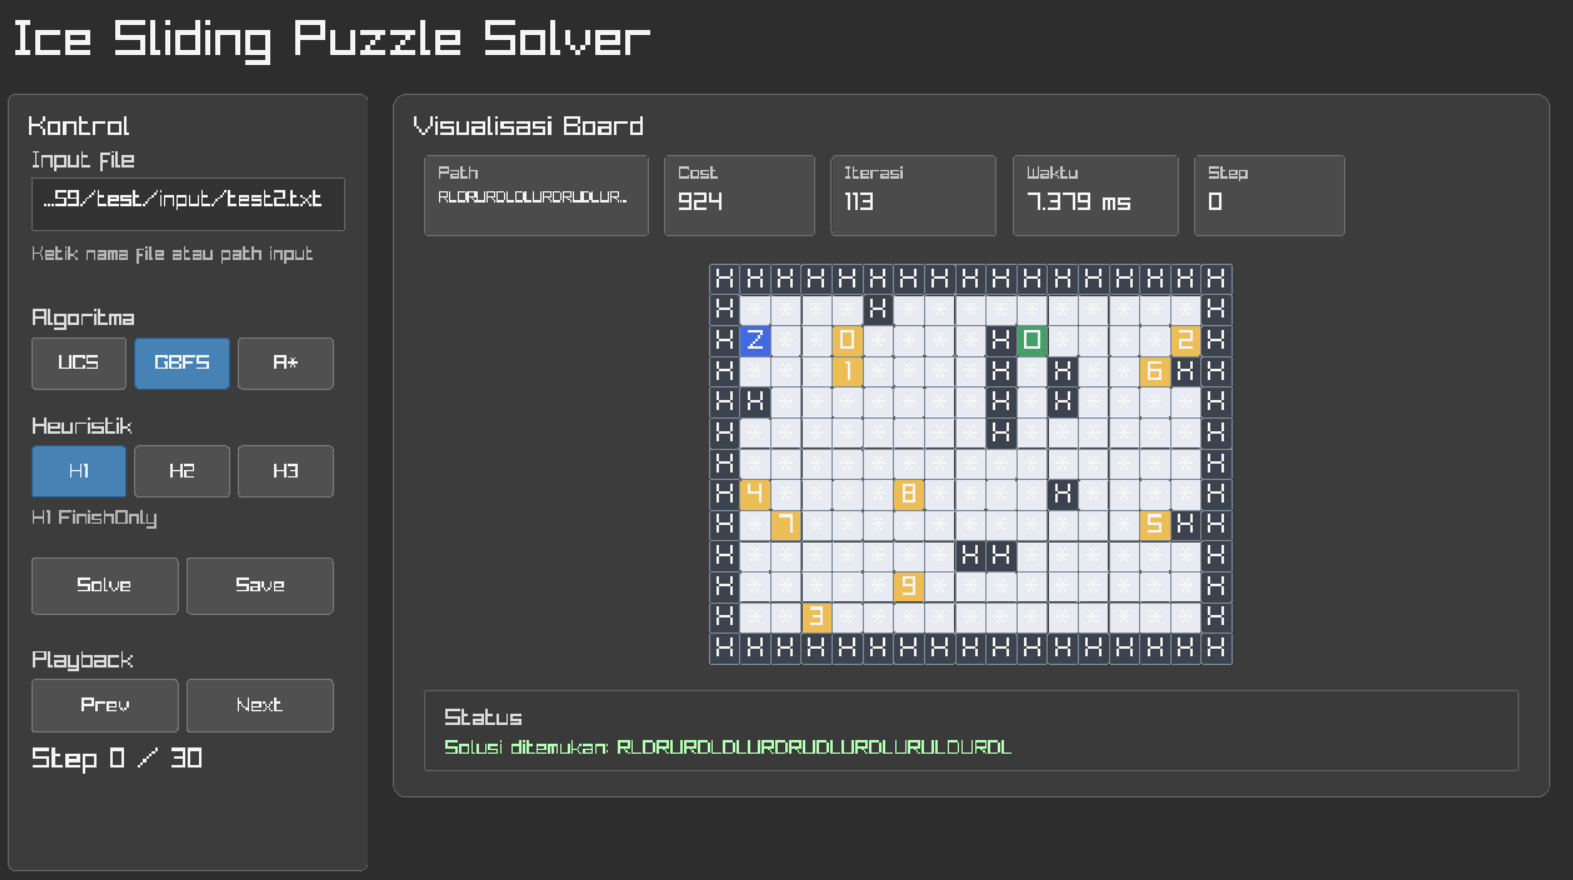
\includegraphics[width=0.85\linewidth]{Screenshot2.png}
    }{
        \fbox{\begin{minipage}[c][3cm][c]{0.82\linewidth}\centering Screenshot GUI: Kasus Uji 2 -- test2.txt (GBFS H1)\end{minipage}}
    }
    \caption{Tampilan GUI kasus uji 2 (\texttt{test2.txt}, GBFS H1).}
\end{figure}

% ===== KASUS UJI 3 =====
\subsection{Kasus Uji 3: \texttt{test2.txt} -- GBFS H2}

\noindent\begin{minipage}[t]{0.52\textwidth}
\begin{lstlisting}[basicstyle=\ttfamily\tiny, numbers=none, title=Input: test2.txt]
13 17
XXXXXXXXXXXXXXXXX
X****X**********X
XZ**0****XO****2X
X***1****X*X**6XX
XX*******X*X****X
X********X******X
X***************X
X4****8****X****X
X*7***********5XX
X*******XX******X
X*****9*********X
X**3************X
XXXXXXXXXXXXXXXXX
999 999 999 999 999 999 999 999 999 999 999 999 999 999 999 999 999
999 9 5 1 6 999 7 3 8 4 9 5 1 6 2 7 999
999 3 8 4 9 5 1 6 2 999 3 8 4 9 5 1 999
999 6 2 7 3 8 4 9 5 999 6 999 7 3 8 999 999
999 999 5 1 6 2 7 3 8 999 9 999 1 6 2 7 999
999 3 8 4 9 5 1 6 2 999 3 8 4 9 5 1 999
999 6 2 7 3 8 4 9 5 1 6 2 7 3 8 4 999
999 9 5 1 6 2 7 3 8 4 9 999 1 6 2 7 999
999 3 8 4 9 5 1 6 2 7 3 8 4 9 5 999 999
999 6 2 7 3 8 4 9 999 999 6 2 7 3 8 4 999
999 9 5 1 6 2 7 3 8 4 9 5 1 6 2 7 999
999 3 8 4 9 5 1 6 2 7 3 8 4 9 5 1 999
999 999 999 999 999 999 999 999 999 999 999 999 999 999 999 999 999
\end{lstlisting}
\end{minipage}%
\hfill%
\begin{minipage}[t]{0.44\textwidth}
\begin{lstlisting}[basicstyle=\ttfamily\scriptsize, numbers=none, title=Output]
Solusi Yang Ditemukan :
  RLDRURDLDLURDRUDL
  URDLURULDURDL
Cost dari Solusi : 924
Initial
XXXXXXXXXXXXXXXXX
X****X**********X
XZ**0****XO****2X
X***1****X*X**6XX
XX*******X*X****X
X********X******X
X***************X
X4****8****X****X
X*7***********5XX
X*******XX******X
X*****9*********X
X**3************X
XXXXXXXXXXXXXXXXX
...
>> Waktu eksekusi: 0.066 ms
>> Banyak iterasi yang dilakukan: 102 iterasi
\end{lstlisting}
\end{minipage}

\begin{figure}[H]
    \centering
    \IfFileExists{screenshot3.png}{
        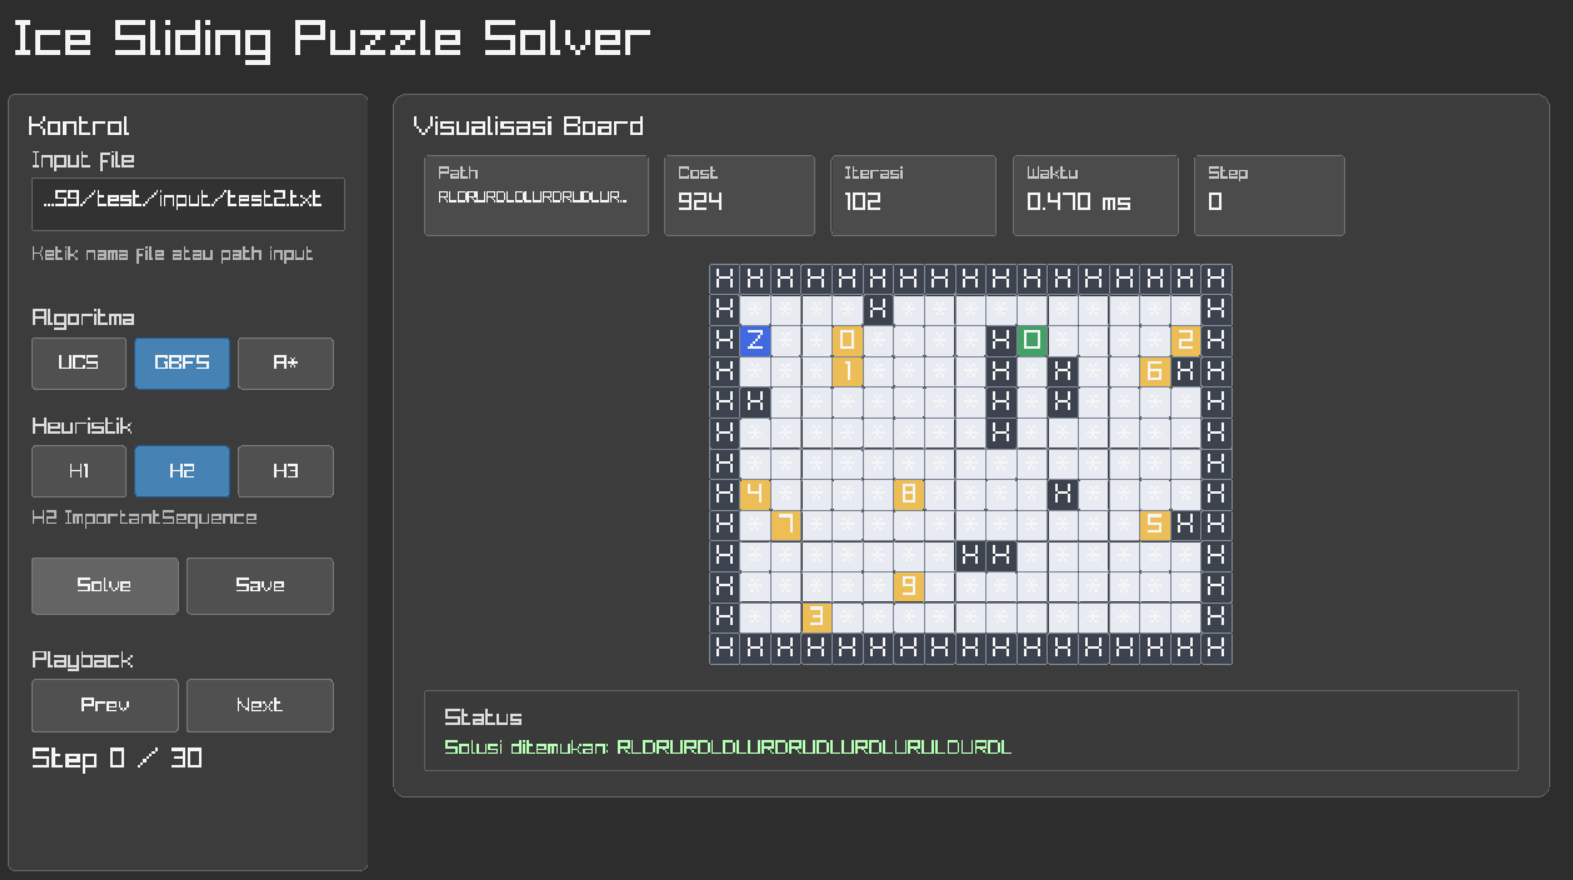
\includegraphics[width=0.85\linewidth]{Screenshot3.png}
    }{
        \fbox{\begin{minipage}[c][3cm][c]{0.82\linewidth}\centering Screenshot GUI: Kasus Uji 3 -- test2.txt (GBFS H2)\end{minipage}}
    }
    \caption{Tampilan GUI kasus uji 3 (\texttt{test2.txt}, GBFS H2).}
\end{figure}

% ===== KASUS UJI 4 =====
\subsection{Kasus Uji 4: \texttt{test3.txt} -- A* H1}

\noindent\begin{minipage}[t]{0.52\textwidth}
\begin{lstlisting}[basicstyle=\ttfamily\tiny, numbers=none, title=Input: test3.txt]
18 26
XXXXXXXXXXXXXXXXXXXXXXXXXX
X************************X
X***X**************X*****X
X************************X
X**4****X****************X
XXX**********************X
X*******************X****X
X**********X*X******X***5X
X*********XX9XX********XXX
X*********ZXO******0*****X
X1**XX****XX8XX****XX****X
X*********3X*X***********X
X***X********************X
XXX********************XXX
X2**********7***********6X
X******X*****************X
X**********X*************X
XXXXXXXXXXXXXXXXXXXXXXXXXX
999 999 999 999 999 999 999 999 999 999 999 999 999 999 999 999 999 999 999 999 999 999 999 999 999 999
999 9 5 1 6 2 7 3 8 4 9 5 1 6 2 7 3 8 4 9 5 1 6 2 7 999
999 3 8 4 999 5 1 6 2 7 3 8 4 9 5 1 6 2 7 999 8 4 9 5 1 999
999 6 2 7 3 8 4 9 5 1 6 2 7 3 8 4 9 5 1 6 2 7 3 8 4 999
999 9 5 1 6 2 7 3 999 4 9 5 1 6 2 7 3 8 4 9 5 1 6 2 7 999
999 999 999 4 9 5 1 6 2 7 3 8 4 9 5 1 6 2 7 3 8 4 9 5 1 999
999 6 2 7 3 8 4 9 5 1 6 2 7 3 8 4 9 5 1 6 999 7 3 8 4 999
999 9 5 1 6 2 7 3 8 4 9 999 1 999 2 7 3 8 4 9 999 1 6 2 7 999
999 3 8 4 9 5 1 6 2 7 999 999 4 999 999 1 6 2 7 3 8 4 9 999 999 999
999 6 2 7 3 8 4 9 5 1 6 999 7 999 8 4 9 5 1 6 2 7 3 8 4 999
999 9 5 1 6 999 999 3 8 4 999 999 1 999 999 7 3 8 4 999 999 1 6 2 7 999
999 3 8 4 9 5 1 6 2 7 3 999 4 999 5 1 6 2 7 3 8 4 9 5 1 999
999 6 2 7 999 8 4 9 5 1 6 2 7 3 8 4 9 5 1 6 2 7 3 8 4 999
999 999 999 1 6 2 7 3 8 4 9 5 1 6 2 7 3 8 4 9 5 1 6 999 999 999
999 3 8 4 9 5 1 6 2 7 3 8 4 9 5 1 6 2 7 3 8 4 9 5 1 999
999 6 2 7 3 8 4 999 5 1 6 2 7 3 8 4 9 5 1 6 2 7 3 8 4 999
999 9 5 1 6 2 7 3 8 4 9 999 1 6 2 7 3 8 4 9 5 1 6 2 7 999
999 999 999 999 999 999 999 999 999 999 999 999 999 999 999 999 999 999 999 999 999 999 999 999 999 999
\end{lstlisting}
\end{minipage}%
\hfill%
\begin{minipage}[t]{0.44\textwidth}
\begin{lstlisting}[basicstyle=\ttfamily\scriptsize, numbers=none, title=Output]
Solusi Yang Ditemukan :
  LURDRDLULUDRDLUDR
  ULDRURDLDRUDLULDR
  DLDRULURDL
Cost dari Solusi : 2452
Initial
XXXXXXXXXXXXXXXXXXXXXXXXXX
X************************X
X***X**************X*****X
X************************X
X**4****X****************X
XXX**********************X
X*******************X****X
X**********X*X******X***5X
X*********XX9XX********XXX
X*********ZXO******0*****X
X1**XX****XX8XX****XX****X
X*********3X*X***********X
X***X********************X
XXX********************XXX
X2**********7***********6X
X******X*****************X
X**********X*************X
XXXXXXXXXXXXXXXXXXXXXXXXXX
...
>> Waktu eksekusi: 0.122 ms
>> Banyak iterasi yang dilakukan: 217 iterasi
\end{lstlisting}
\end{minipage}

\begin{figure}[H]
    \centering
    \IfFileExists{Screenshot4.png}{
        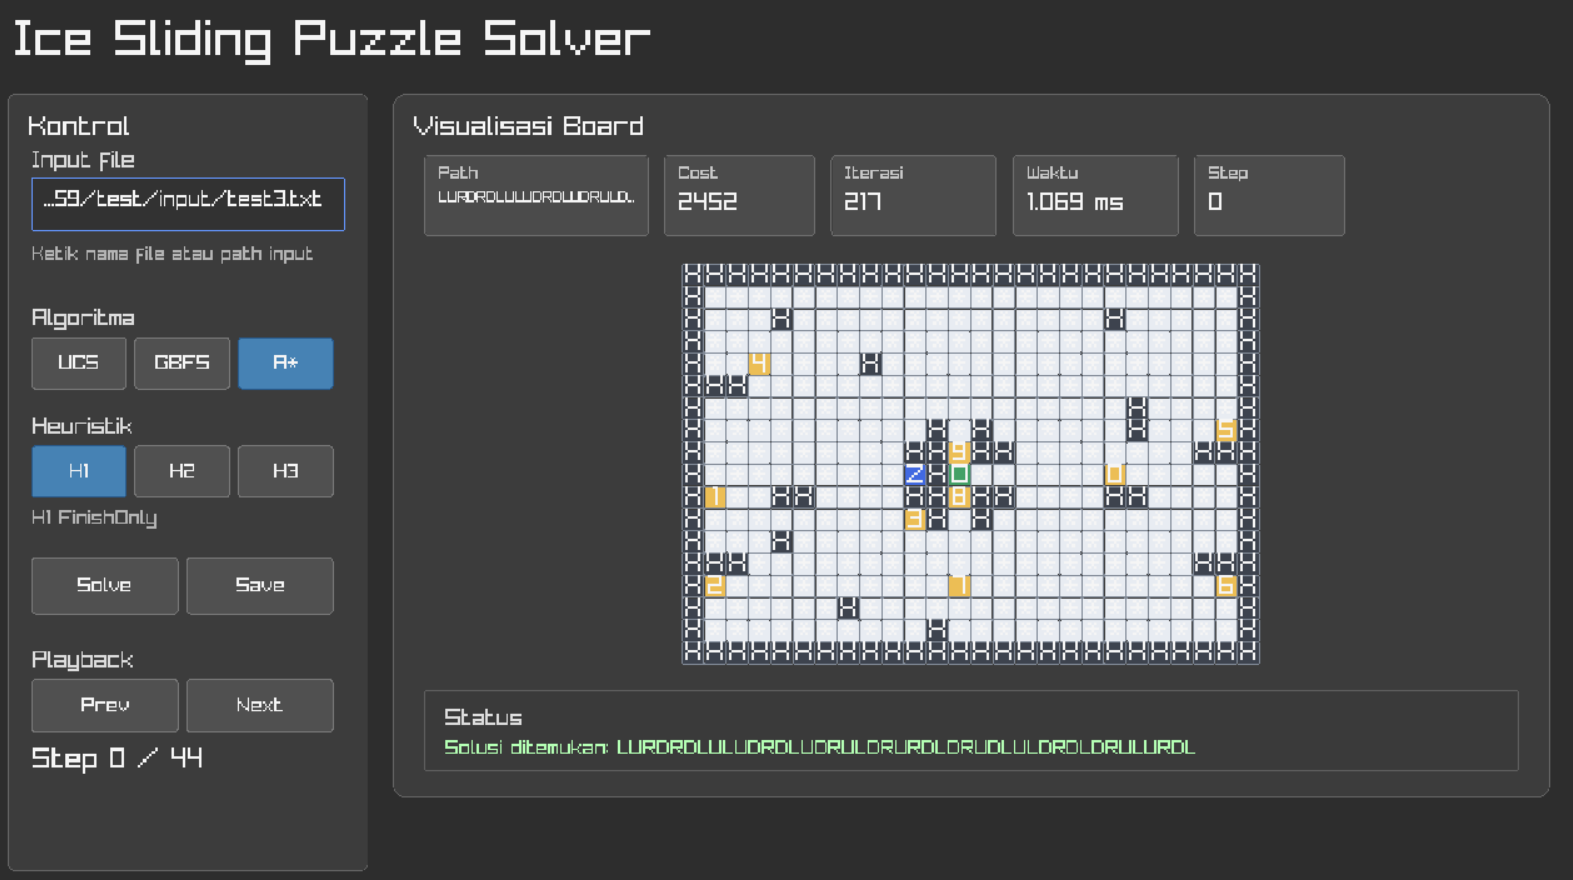
\includegraphics[width=0.85\linewidth]{Screenshot4.png}
    }{
        \fbox{\begin{minipage}[c][3cm][c]{0.82\linewidth}\centering Screenshot GUI: Kasus Uji 4 -- test3.txt (A* H1)\end{minipage}}
    }
    \caption{Tampilan GUI kasus uji 4 (\texttt{test3.txt}, A* H1).}
\end{figure}

% ===== KASUS UJI 5 =====
\subsection{Kasus Uji 5: \texttt{test3.txt} -- A* H3}

\noindent\begin{minipage}[t]{0.52\textwidth}
\begin{lstlisting}[basicstyle=\ttfamily\tiny, numbers=none, title=Input: test3.txt]
18 26
XXXXXXXXXXXXXXXXXXXXXXXXXX
X************************X
X***X**************X*****X
X************************X
X**4****X****************X
XXX**********************X
X*******************X****X
X**********X*X******X***5X
X*********XX9XX********XXX
X*********ZXO******0*****X
X1**XX****XX8XX****XX****X
X*********3X*X***********X
X***X********************X
XXX********************XXX
X2**********7***********6X
X******X*****************X
X**********X*************X
XXXXXXXXXXXXXXXXXXXXXXXXXX
999 999 999 999 999 999 999 999 999 999 999 999 999 999 999 999 999 999 999 999 999 999 999 999 999 999
999 9 5 1 6 2 7 3 8 4 9 5 1 6 2 7 3 8 4 9 5 1 6 2 7 999
999 3 8 4 999 5 1 6 2 7 3 8 4 9 5 1 6 2 7 999 8 4 9 5 1 999
999 6 2 7 3 8 4 9 5 1 6 2 7 3 8 4 9 5 1 6 2 7 3 8 4 999
999 9 5 1 6 2 7 3 999 4 9 5 1 6 2 7 3 8 4 9 5 1 6 2 7 999
999 999 999 4 9 5 1 6 2 7 3 8 4 9 5 1 6 2 7 3 8 4 9 5 1 999
999 6 2 7 3 8 4 9 5 1 6 2 7 3 8 4 9 5 1 6 999 7 3 8 4 999
999 9 5 1 6 2 7 3 8 4 9 999 1 999 2 7 3 8 4 9 999 1 6 2 7 999
999 3 8 4 9 5 1 6 2 7 999 999 4 999 999 1 6 2 7 3 8 4 9 999 999 999
999 6 2 7 3 8 4 9 5 1 6 999 7 999 8 4 9 5 1 6 2 7 3 8 4 999
999 9 5 1 6 999 999 3 8 4 999 999 1 999 999 7 3 8 4 999 999 1 6 2 7 999
999 3 8 4 9 5 1 6 2 7 3 999 4 999 5 1 6 2 7 3 8 4 9 5 1 999
999 6 2 7 999 8 4 9 5 1 6 2 7 3 8 4 9 5 1 6 2 7 3 8 4 999
999 999 999 1 6 2 7 3 8 4 9 5 1 6 2 7 3 8 4 9 5 1 6 999 999 999
999 3 8 4 9 5 1 6 2 7 3 8 4 9 5 1 6 2 7 3 8 4 9 5 1 999
999 6 2 7 3 8 4 999 5 1 6 2 7 3 8 4 9 5 1 6 2 7 3 8 4 999
999 9 5 1 6 2 7 3 8 4 9 999 1 6 2 7 3 8 4 9 5 1 6 2 7 999
999 999 999 999 999 999 999 999 999 999 999 999 999 999 999 999 999 999 999 999 999 999 999 999 999 999
\end{lstlisting}
\end{minipage}%
\hfill%
\begin{minipage}[t]{0.44\textwidth}
\begin{lstlisting}[basicstyle=\ttfamily\scriptsize, numbers=none, title=Output]
Solusi Yang Ditemukan :
  LURDRDLULUDRDLUDR
  ULDRURDLDRUDLULDR
  DLDRULURDL
Cost dari Solusi : 2452
Initial
XXXXXXXXXXXXXXXXXXXXXXXXXX
X************************X
X***X**************X*****X
X************************X
X**4****X****************X
XXX**********************X
X*******************X****X
X**********X*X******X***5X
X*********XX9XX********XXX
X*********ZXO******0*****X
X1**XX****XX8XX****XX****X
X*********3X*X***********X
X***X********************X
XXX********************XXX
X2**********7***********6X
X******X*****************X
X**********X*************X
XXXXXXXXXXXXXXXXXXXXXXXXXX
...
>> Waktu eksekusi: 0.122 ms
>> Banyak iterasi yang dilakukan: 217 iterasi
\end{lstlisting}
\end{minipage}

\begin{figure}[H]
    \centering
    \IfFileExists{Screenshot5.png}{
        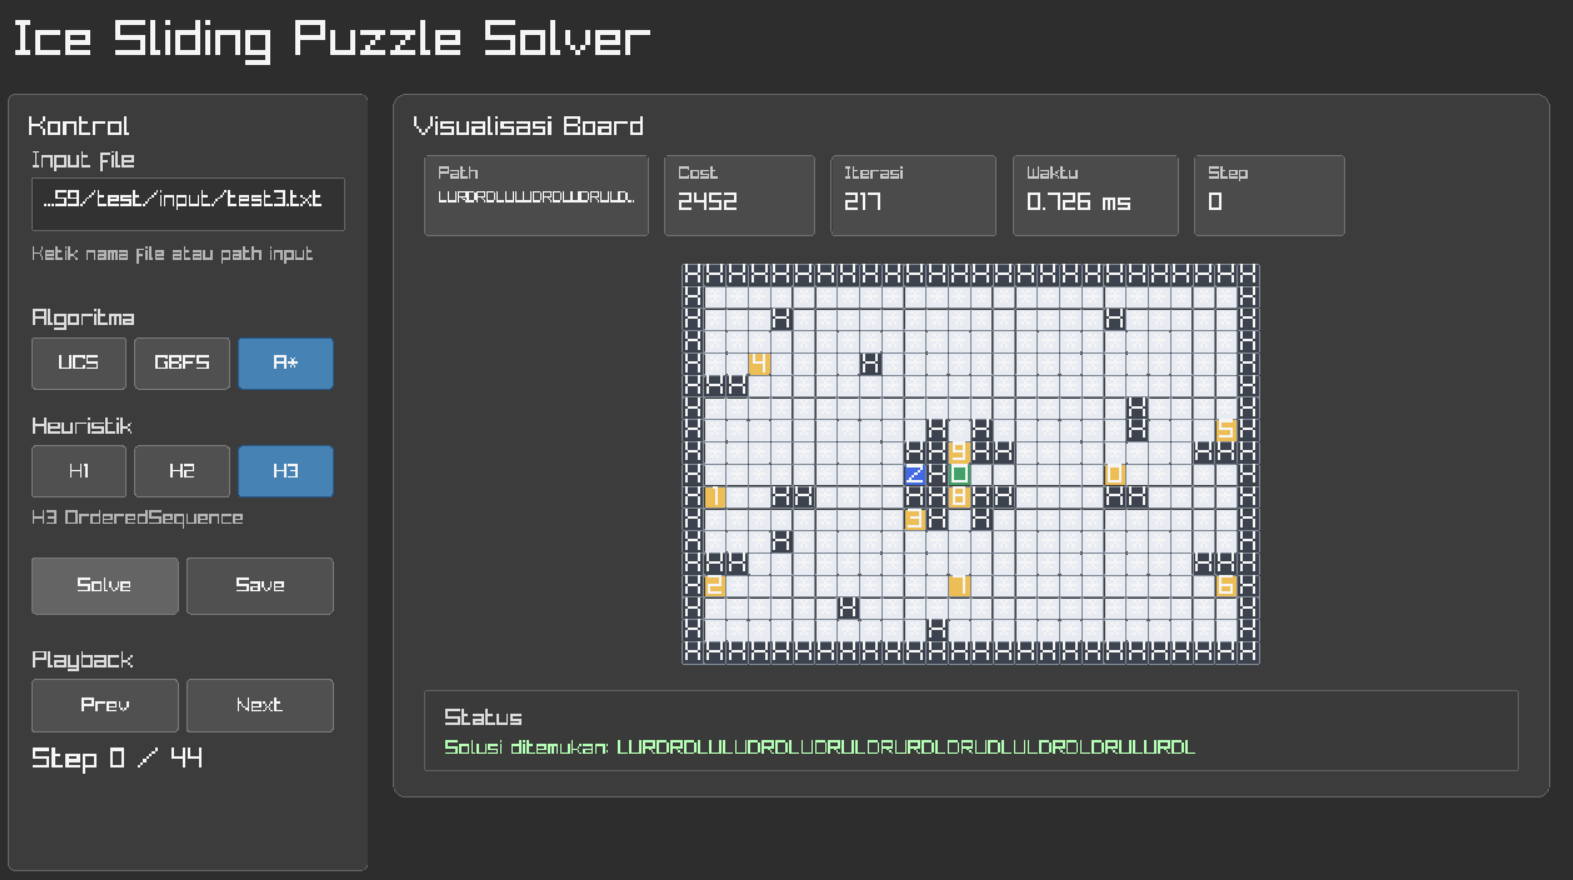
\includegraphics[width=0.85\linewidth]{Screenshot5.png}
    }{
        \fbox{\begin{minipage}[c][3cm][c]{0.82\linewidth}\centering Screenshot GUI: Kasus Uji 5 -- test3.txt (A* H3)\end{minipage}}
    }
    \caption{Tampilan GUI kasus uji 5 (\texttt{test3.txt}, A* H3).}
\end{figure}

\subsection{Analisis Hasil Percobaan}

Tabel berikut merangkum hasil seluruh kasus uji yang telah dilakukan.

\begin{longtable}{|p{1cm}|p{2cm}|p{2.2cm}|p{5cm}|p{1.3cm}|p{1.5cm}|}
    \hline
    \textbf{Uji} & \textbf{File} & \textbf{Algoritma} & \textbf{Path} & \textbf{Cost} & \textbf{Iterasi} \\
    \hline
    \endhead
    1 & test1.txt & UCS &
        {\ttfamily\footnotesize RULUDRUR} & 87 & 13 \\
    \hline
    2 & test2.txt & GBFS H1 &
        {\ttfamily\footnotesize RLDRURDLDLURDRUDL\newline URDLURULDURDL} & 924 & 113 \\
    \hline
    3 & test2.txt & GBFS H2 &
        {\ttfamily\footnotesize RLDRURDLDLURDRUDL\newline URDLURULDURDL} & 924 & 102 \\
    \hline
    4 & test3.txt & A* H1 &
        {\ttfamily\footnotesize LURDRDLULUDRDLUDR\newline ULDRURDLDRUDLULDR\newline DLDRULURDL} & 2452 & 217 \\
    \hline
    5 & test3.txt & A* H3 &
        {\ttfamily\footnotesize LURDRDLULUDRDLUDR\newline ULDRURDLDRUDLULDR\newline DLDRULURDL} & 2452 & 217 \\
    \hline
\end{longtable}

\section{Kesimpulan dan Saran}
\subsection{Kesimpulan}

Permainan Ice Sliding Puzzle dapat dimodelkan sebagai persoalan pencarian jalur pada graph sederhana, di mana setiap node mewakili posisi berhenti aktor dan setiap edge mewakili satu gerakan sliding lengkap beserta cost akumulatif dan daftar tile penting yang dilewati. Pendekatan ini memungkinkan representasi yang ringkas karena hanya posisi-posisi yang benar-benar dapat menjadi tempat berhenti yang dijadikan node, bukan seluruh tile pada papan.

Aturan urutan tile angka ditangani dengan memperluas definisi state pencarian menjadi pasangan $(nodeId, nextNumber)$. Dengan demikian, dua kunjungan ke posisi yang sama dengan progres angka yang berbeda diperlakukan sebagai dua state yang berbeda dan tidak saling menggugurkan. Mekanisme tabel \texttt{bestCost} berperan sebagai pruning untuk mencegah ekspansi ulang state dengan cost yang lebih buruk.

Ketiga algoritma UCS, GBFS, dan A* dapat diimplementasikan dalam satu fungsi pencarian yang sama, dengan perbedaan hanya pada formula prioritas. UCS menggunakan $g(n)$ saja sehingga menjamin solusi optimal selama cost edge tidak negatif. GBFS menggunakan $h(n)$ saja sehingga lebih cepat menemukan solusi tetapi tidak ada jaminan optimalitas. A* menggabungkan keduanya dengan $f(n) = g(n) + h(n)$, menjamin optimalitas apabila heuristic yang digunakan bersifat admissible.

Heuristic berbasis jarak Manhattan tidak selalu admissible pada permainan sliding karena satu gerakan dapat melewati banyak tile sekaligus dengan cost kumulatif yang berbeda-beda dari estimasi Manhattan. Meskipun demikian, pada sebagian besar peta uji ketiga heuristic H1, H2, dan H3 tetap memberikan panduan arah pencarian yang efektif sehingga A* maupun GBFS dapat menemukan solusi yang optimal atau mendekati optimal dalam jumlah iterasi yang jauh lebih sedikit dibanding UCS.

\subsection{Saran}
Beberapa saran pengembangan program di masa mendatang adalah sebagai berikut.
\begin{enumerate}
    \item Heuristic dapat dikembangkan agar lebih informatif dan tetap admissible, misalnya dengan mempertimbangkan struktur rintangan dan cost minimum tile pada peta.
    \item Visualisasi GUI dapat diperluas dengan animasi pergerakan aktor dan penanda jalur yang sudah ditelusuri agar pengguna lebih mudah memahami solusi.
    \item Dukungan format input dapat diperluas, misalnya dengan menambahkan validasi yang lebih informatif terhadap kesalahan format file.
    \item Algoritma pencarian dapat diperluas dengan varian seperti IDA* atau Bidirectional Search untuk dibandingkan performanya pada peta berukuran lebih besar.
\end{enumerate}

\section{Daftar Pustaka}
\begin{enumerate}
    \item Munir, R. (2026). \textit{Route Planning (Bagian 1)}. Program Studi Teknik Informatika, Sekolah Teknik Elektro dan Informatika, Institut Teknologi Bandung. \url{https://informatika.stei.itb.ac.id/~rinaldi.munir/Stmik/2025-2026/21-Route-Planning-(2026)-Bagian1.pdf}.
    \item Munir, R. (2026). \textit{Route Planning (Bagian 2)}. Program Studi Teknik Informatika, Sekolah Teknik Elektro dan Informatika, Institut Teknologi Bandung. \url{https://informatika.stei.itb.ac.id/~rinaldi.munir/Stmik/2025-2026/22-Route-Planning-(2026)-Bagian2.pdf}.
    \item Russell, S., \& Norvig, P. (2020). \textit{Artificial Intelligence: A Modern Approach} (4th ed.). Pearson.
    \item Cormen, T. H., Leiserson, C. E., Rivest, R. L., \& Stein, C. (2022). \textit{Introduction to Algorithms} (4th ed.). MIT Press.
    \item Dokumentasi resmi raylib. \url{https://www.raylib.com/}.
\end{enumerate}

\newpage
\section{Lampiran}

\begin{table}[H]
    \centering
    \renewcommand{\arraystretch}{1.5}
    \begin{tabular}{|c|p{9.5cm}|c|c|}
        \hline
        \textbf{No} & \textbf{Poin} & \textbf{Ya} & \textbf{Tidak} \\
        \hline
        1 & Program berhasil di kompilasi tanpa kesalahan & $\checkmark$ &  \\
        \hline
        2 & Program berhasil dijalankan & $\checkmark$ &  \\
        \hline
        3 & Solusi yang diberikan program benar dan mematuhi aturan permainan & $\checkmark$ &  \\
        \hline
        4 & Program dapat membaca masukan berkas \texttt{.txt} serta menyimpan solusi dalam berkas \texttt{.txt} & $\checkmark$ &  \\
        \hline
        5 & Program memiliki Graphical User Interface (GUI) & $\checkmark$ &  \\
        \hline
        6 & Ada algoritma \textit{pathfinding} alternatif selain dari spesifikasi wajib (Algoritma X dan Algoritma Y) &  & $\checkmark$ \\
        \hline
        7 & Ada tambahkan dua alternatif heuristik selain yang utama (Heuristik X dan Heuristik Y) & $\checkmark$ &  \\
        \hline
    \end{tabular}
\end{table}

\vspace{1cm}
\noindent
\fbox{
\begin{minipage}{0.97\linewidth}
Tugas ini disusun sepenuhnya tanpa bantuan kecerdasan buatan (Generative AI), 
melainkan hasil pemikiran dan analisis mandiri. 

\begin{flushright}
\IfFileExists{ttd.png}{
    \includegraphics[height=2cm,keepaspectratio]{ttd.png}\\
}{
    \vspace{2cm}
}
Raymond Jonathan Dwi Putra Julianto
\end{flushright}
\end{minipage}%
}

\vspace{1cm}
\noindent
\textbf{Tautan Repositori:} \url{https://github.com/Alpaomega1136/Tucil3_13524059}

\end{document}